\documentclass[../report.tex]{subfiles}

\begin{document}
\subsection{Giới thiệu về hàm băm mật mã MD5}
MD5 là một hàm băm mật mã học được sử dụng phổ biến với giá trị băm dàm 128 bit. Là một chuẩn Internet (Được mô tả trong RFC 1321). 
MD5 đã được dùng nhiều trong ứng dụng bảo mật, và được sử dụng để kiểm tra tính toàn vẹn của tệp tin. 

MD5 chuyển một đoạn thông tin chiều dài bất kì thành một kết quả có chiều dài không đổi 128 bit. 
MD5 chia tin đầu vào thành từng đoạn 512 bit, được padding thêm để chiều dài nó chia chẵn cho 512. 
Bit 1 được gắn vào cuối mẩu tin đầu vào, sau đó là một dãy số 0, và cuối cùng là một giá trị nguyên không dấu 
64 bit theo kiểu little endian. 

Giải thuật MD5 hoạt động trên trạng thái 128 bit, được chia thành 4 từ 32 bit, kí hiệu là A, B, C, D. Chúng được 
khởi tạo bằng những hằng số cố định. 
Từng gói tin 512 bit được xử lý thông qua bốn giai đoạn, 
mỗi gian đoạn lại bao gồm 16 tác vụ với hàm phi tuyến F giống nhau. 

\begin{figure}[H]
\centering
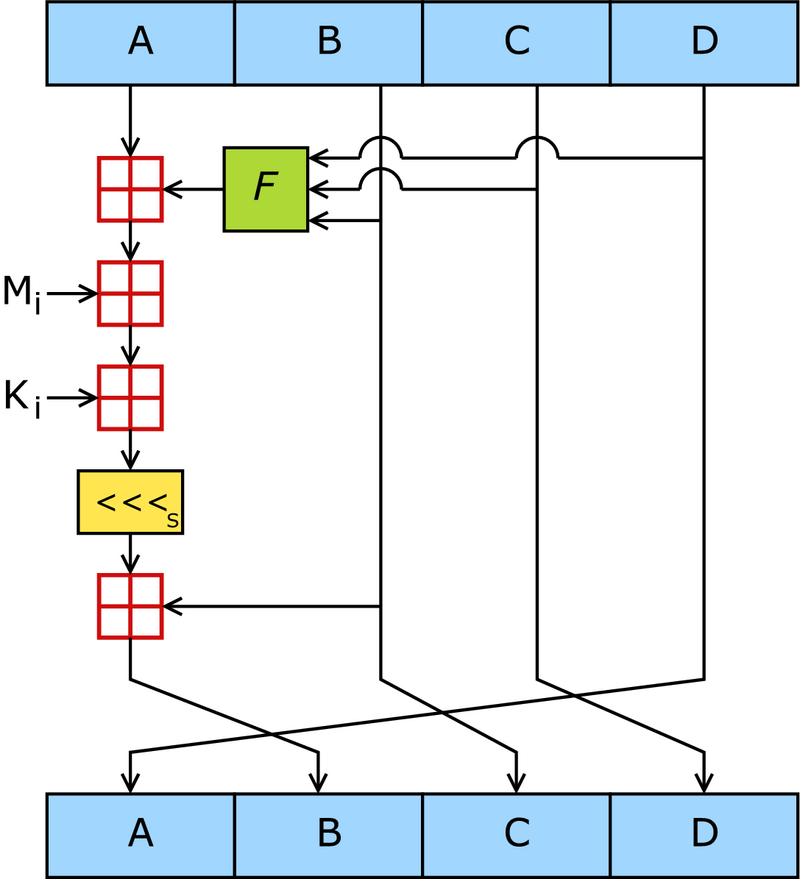
\includegraphics[width=10cm]{figures/md5-diagram.png}
\caption{Một tác vụ trong 64 tác vụ của MD5, trong đó F là một hàm phi tuyến (có 4 hàm phi tuyến), 
ô vuông là phép cộng modulo $2^{32}$, $M_j$ là khối tin đầu vào 32 bit, $K_i$ là hằng số 32 bit, 
mỗi tác vụ có một i j khác nhau, $\lll$ là phép xoay trái.}
\end{figure}

\subsection{Mã C++ của thuật toán MD5}
\lstset{language=C++,
                basicstyle=\ttfamily,
                keywordstyle=\color{blue}\ttfamily,
                stringstyle=\color{red}\ttfamily,
                commentstyle=\color{green}\ttfamily,
                morecomment=[l][\color{magenta}]{\#}
}
\begin{lstlisting}
#include <iostream>
#include <string>

using word = unsigned int;
using byte = unsigned char;

#define MESSAGE_SIZE 64
#define WORD_COUNT (MESSAGE_SIZE / 4)

byte input[MESSAGE_SIZE];

byte output[WORD_COUNT];

word T[] = {
    0xd76aa478, 0xe8c7b756, 0x242070db, 0xc1bdceee,
    0xf57c0faf, 0x4787c62a, 0xa8304613, 0xfd469501,
    0x698098d8, 0x8b44f7af, 0xffff5bb1, 0x895cd7be,
    0x6b901122, 0xfd987193, 0xa679438e, 0x49b40821,
    0xf61e2562, 0xc040b340, 0x265e5a51, 0xe9b6c7aa,
    0xd62f105d, 0x02441453, 0xd8a1e681, 0xe7d3fbc8,
    0x21e1cde6, 0xc33707d6, 0xf4d50d87, 0x455a14ed,
    0xa9e3e905, 0xfcefa3f8, 0x676f02d9, 0x8d2a4c8a,
    0xfffa3942, 0x8771f681, 0x6d9d6122, 0xfde5380c,
    0xa4beea44, 0x4bdecfa9, 0xf6bb4b60, 0xbebfbc70,
    0x289b7ec6, 0xeaa127fa, 0xd4ef3085, 0x04881d05,
    0xd9d4d039, 0xe6db99e5, 0x1fa27cf8, 0xc4ac5665,
    0xf4292244, 0x432aff97, 0xab9423a7, 0xfc93a039,
    0x655b59c3, 0x8f0ccc92, 0xffeff47d, 0x85845dd1,
    0x6fa87e4f, 0xfe2ce6e0, 0xa3014314, 0x4e0811a1,
    0xf7537e82, 0xbd3af235, 0x2ad7d2bb, 0xeb86d391,
};

void init_input(const std::string& s) {
    size_t i = 0;
    size_t input_size = s.size();
    
    for (; i < input_size; i++)
        input[i] = s[i];
    for (; i < MESSAGE_SIZE; i++)
        input[i] = 0;
    
    input[input_size] = 128;
    word *len = (word *)&input[MESSAGE_SIZE - 8];
    *len = input_size * 8;
}

#define ROTATE_LEFT(x, n) \
    ((x) << (n) | (x) >> (32 - (n)))

void md5() {
    word A = 0x67452301;
    word B = 0xefcdab89;
    word C = 0x98badcfe;
    word D = 0x10325476;

    word *X = (word *)input;

    word AA = A;
    word BB = B;
    word CC = C;
    word DD = D;

    const word s[] = {
        7, 12, 17, 22, 
        5,  9, 14, 20,
        4, 11, 16, 23,
        6, 10, 15, 21,
    };

    for (int i = 0; i < 64; i++) {
        word F, g;
        if (i < 16) {
            F = (B & C) | (~B & D);
            g = i % 16;
        }
        else if (i < 32) {
            F = (D & B) | (~D & C);
            g = (5*i + 1) % 16;
        }
        else if (i < 48) {
            F = B ^ C ^ D;
            g = (3*i + 5) % 16;
        }
        else {
            F = C ^ (B | ~D);
            g = (7*i) % 16;
        }
        
        F = F + A + X[g] + T[i]; 
        A = D;
        D = C;
        C = B;
        B += ROTATE_LEFT(F, s[(i / 16) * 4 + i % 4]);
    }
    A += AA;
    B += BB;
    C += CC;
    D += DD;

    ((word *)output)[0] = A;
    ((word *)output)[1] = B;
    ((word *)output)[2] = C;
    ((word *)output)[3] = D;
}

void print_output() {
    for (byte b: output)
        std::cout << std::hex << (word)b << std::endl;
}

int main() {
    init_input("abcd");
    md5();
    print_output();

    return 0;
}
\end{lstlisting}

\noindent Code thực hiện trên assembly dựa theo code C++ này. 


\end{document}
